
% The API of \sys\ is presented in Section~\ref{ssec:api}. 
\cref{ssec:layout}  discusses \sys's data organization. 
We discuss
atomic scans  in \cref{ssec:scans}, and describe \sys's
 normal (maintenance-free) operation flow  in \cref{ssec:ops}.  
The data structure's maintenance is discussed in \cref{ssec:rebalance}.
Finally, \cref{ssec:flush-recovery} discusses flushing data to disk and failure recovery.


\subsection{Data organization}
\label{ssec:layout}


\paragraph{Chunks, funks, and munks.}

\sys's data layout is depicted in Figure~\ref{fig:piwi}.
%Similarly to BTrees and other disk-friendly and cache-friendly data structures~\cite{kiwi}, 
Data resides in chunks, each holding a contiguous key range.
This improves the efficiency of both disk access and memory access, in particular, for  range scans. 
Each chunk's data 
(consisting of keys in the corresponding range and values associated with them) 
is kept on disk (funks, for persistence), and possibly in memory (munks, for fast access). 
Chunk's metadata objects are significantly smaller than munks and funks
(typically, less than 1 KB instead of tens of MBs). Hence, at run-time, \sys\ holds in memory a list of all metadata objects.
In addition, it keeps a volatile \emph{chunk index} -- a sorted map from keys to chunks. 
Index updates are lazy, so it only offers best-effort expedited search.

On disk, each chunk is associated with a funk, % as illustrated in Figure~\ref{fig:funk}. 
consisting of two files:  a compacted and sorted  key-value map \emph{SSTable} (Sorted String Table~\cite{Bigtable2008}) 
and a write \emph{log}. When a funk is created, the \code{SSTable} holds all the chunk's keys with corresponding values, and the \code{log}  is empty.
New key-value pairs are subsequently appended to the unsorted \code{log}. If a key is over-written, it remains in the \code{SSTable} associated with the old value, and is included in the \code{log} with the new one.
That is, the \code{log} is more up-to-date.

\remove{
\begin{figure}[tb]
\centerline{
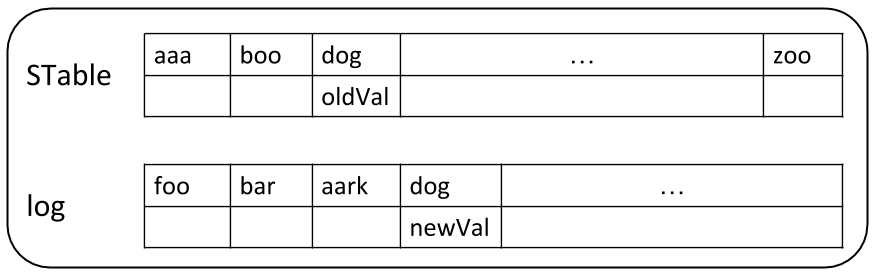
\includegraphics[width=\columnwidth]{funk.png}
}
\caption{A \sys\ funk consists of a sorted \code{SSTable} and an unsorted \code{log} holding the most recent updates.}
\label{fig:funk}
\end{figure}
}

This structure allows us to benefit from sorted searches on the \code{SSTable}, and at the same time
allows for updating chunks without re-writing existing data, thus minimizing write amplification.
As a funk's \code{log}  grows, however, searching becomes inefficient   and  
the funk is no longer compact, i.e., it may contain redundant (over-written) values.
Therefore, once the \code{log}  exceeds a certain threshold, we reorganize the funk
via a process we call \emph{rebalance}, as explained below.
\remove{
In our experiments, we keep the \code{log} \inred{an order of magnitude smaller than \emph{or} 
around the same size as?} the \code{SSTable}  .
}

A subset of the chunks is also cached in memory to allow fast access, the content of where each cached chunk is stored in a
munk data structure. 
Munks are volatile and can be removed and recreated from funks at any time based on an arbitrary replacement policy.
% Thus, multiple \emph{generations} of munks may exist for a chunk throughout its life time.
%Chunks that are not cached are denoted \emph{munk-less}.

%The details of the chunk's metadata structure are deferred to the the supplemental material.

A munk holds key-value pairs in an array-based linked list.  
\remove{
A munk consists of two arrays -- \emph{karray} for keys and \emph{varray} for values. The  \code{karray}  holds a sorted linked list of the chunk's keys
with pointers to values in the \code{varray}. 
}
When a munk is created, some prefix of this array is populated,
sorted by key, so each cell's successor in the linked list is the ensuing cell in the array.
New key-value entries are appended after this prefix.
As new entries are added, they create bypasses in the linked list, and consecutive keys in the
list are no longer necessarily adjacent in the array. Nevertheless, as long as 
a sizable prefix of the  array  is sorted, bypasses are short in expectation.
\remove{Key removals, in turn, leave obsolete values in the munk, so it is no longer compacted.}
Keys can thus be searched efficiently via binary search on the sorted prefix followed by a short traversal of a bypass path at the suffix of the array. 


As key-value pairs are added, overwritten, and removed munks and funks need to undergo reorganization. This includes  
(1) \emph{compaction} to garbage-collect removed and overwritten data, 
(2) \emph{sorting} keys to make searches more efficient,  and
(3) \emph{splitting} overflowing chunks.
All reorganizations are performed by \sys's \emph{rebalance} operation.
If the chunk has a munk, then rebalance compacts and sorts the munk in-memory by creating a new 
(compacted and sorted) munk instead of the existing one. 
Funks are also compacted and replaced by new funks, albeit less frequently.
Splits  create new chunks as well as new  funks (and possibly munks) associated with them.

\paragraph{Expediting reads.}
As long as a chunk  is memory-resident, the munk data structure serves both the read-path and the write-path for keys in this chunk's range. 
In this case, the chunk metadata is quickly located using the index, and its munk's sorted prefix allows for fast binary search.
Thus, \sys\ is particularly fast when almost the entire working set is memory-resident. 
We take two measures to mitigate the performance penalty of accessing keys in non cached chunks.

First, we keep a \emph{row cache} holding popular key-value pairs from munk-less chunks. Note that unlike munks, which cache key ranges, the row
cache holds individual keys, and is thus more effective in dealing with point queries (gets as opposed to scans) with no
spatial locality.
Whereas, popular key ranges %are associated with munks (and 
can be scanned quickly from munks, 
isolated hot keys %are included in the row cache for efficient gets.
can be quickly found using the row cache.

For working sets that are  larger than the available DRAM, these two caches might not suffice, and so a certain portion of reads are served from disk. Here, the slowest step is the sequential search of the \code{log}. 
%If an uncached key indeed resides in the 
%\code{log} we need to locate it in the \code{log} in order to find 
%its associated value. 
To reduce \code{log} searches to a minimum,
each munk-less chunk holds a \emph{Bloom filter} for the corresponding funk's \code{log}.
\remove{this is a statistical data structure that summarizes a set of keys so that 
when queried for a key that is included in it always returns true (no false negatives), 
and otherwise returns false with some high probability (low false positive probability).}
Using Bloom filters, we eliminate most of the redundant \code{log}  searches.
To reduce the \code{log} search time in case it does happen, 
we further  partition the Bloom filter into a  handful of filters, each summarizing the 
content of part of the \code{log}; this allows us to know not only whether or not to search the 
\code{log}, but also which part of it to search.  
 
\remove{
\paragraph{Chunk metadata structure.}

The metadata structure is given in Algorithm~\ref{alg:chunk}. 
The first field is its \code{status}, which is explained in \cref{ssec:rebalance}  below. 
It next holds a pointer to the appropriate funk, and either a munk or a Bloom filter, as well as a pointer to the next 
chunk in the chunk linked list.
\remove{
It further keeps the generation number of its latest munk, \code{gen}, and a per-generation sequence number,
\code{seq}, which, in case there is an active munk, is the index of the next free cell in the munk's  \code{karray}  and \code{varray}. The chunk's \code{gen} and \code{seq} are stored together in one 64-bit word to allow 
atomic access to both of them. 
}
%It further includes a Bloom filter as explained above.
Finally, the chunk includes locks to synchronize concurrent access by multiple threads, as explained below.

\begin{algorithm}[htb]

\begin{algorithmic}
\State \code{status} \Comment  baby, child, active, asleep, or aged
\State ptr \code{funk} \Comment funk disk address
\State ptr \code{munk} \Comment munk memory pointer
\State ptr \code{next} \Comment next chunk in linked list
%\State int \code{gen} \Comment munk generation
%\State int \code{seq} \Comment sequence number in current generation 
\State ptr \code{bloomFilter} \Comment summary of set of keys in \code{log}
\State asymmetric lock \code{rebalanceLock} \Comment shared/exclusive lock 
\State lock \code{funkChangeLock} \Comment acquired with try\_lock 
% \State \code{$\langle$key, version, done, counter$\rangle$  PPA[threads]} \Comment pending puts
\end{algorithmic}

\caption{Chunk metadata structure.}
\label{alg:chunk}
\end{algorithm}
}

\paragraph{Thread synchronization variables.}

\sys\ supports concurrent execution of all operations.
The replacement of a chunk (due to a split) or rebalance of a funk or munk %(see Section~\ref{ssec:rebalance}) %associated with a given chunk 
must be executed atomically, and moreover, must be synchronized with concurrent puts. 
This is controlled by the chunk's \emph{rebalanceLock}, which is held for short time periods
during chunk, funk, and munk replacements.  It is a shared/exclusive lock, acquired in shared mode by puts and in exclusive mode by rebalance. Gets and scans do not acquire the lock.

Rebalance makes the new chunk accessible after it is populated. Because a chunk is immutable during rebalance (thanks to rebalance lock), reading either the old or the new version is acceptable.

To minimize I/O, we allow at most one thread to rebalance a funk at a given time; this is controlled by 
the  \code{funkChangeLock}. 
This lock is held throughout the creation of the new funk. 
It is acquired using a try\_lock call, and threads that fail to acquire it do not retry, but instead wait for the winning thread to complete the funk's creation.
%Finally, the chunk holds a data structure called PPA for synchronizing  puts with concurrent scans, as explained in the next section. 

In addition to the chunk list and chunk index, \sys\ keeps a \emph{global version (GV)} for supporting atomic scans (described in the next section) and tracks active threads' activities in the 
\emph{Pending Operations (PO)} array, which has one entry per active thread. 
The PO is used to synchronize puts with scans, as well as for  garbage collection purposes (old 
versions not needed by any active scan can be reclaimed).
We note that using a single pending array to synchronize all operations can cause contention, which we
mitigate in our implementation by tracking the pending puts in per-chunk arrays with per-thread entries as done in~\cite{kiwi}.
%(see the supplemental material for details).%~\cref{sec:impl}). 

\subsection{Multi-versioning for atomic scans}
\label{ssec:scans}

% \paragraph{Multi-versioning.}

We support atomic scans via multi-versioning using the system-wide global version, GV. 
A scan operation creates a \emph{snapshot} associated with GV's current value by incrementing GV, 
which signals to ensuing put operations that they must not overwrite values associated with 
smaller versions than the new GV value.
This resembles a \emph{copy-on-write} approach, which virtually creates a snapshot by 
indicating that data pertaining to the snapshot should not be modified in place.  

To allow garbage collection of old versions, \sys\  tracks snapshot times of 
active scans in the pending operations array, PO.
The compaction process that runs as part of rebalance removes old versions that are no longer required for any  
scan listed in PO. Specifically, for each key, it removes all but the last version that is smaller than the minimal
scan entry in PO and also smaller than the value of GV when the rebalance begins. 

\remove{
For linearizing (i.e., determining an order on) updates, we associate each key-value pair written to the data store 
with a unique-per-key timestamp.
This timestamp is composed as a tuple $\langle$ver, gen, seq$\rangle$, where \emph{ver} is  the version read from GV 
(recall that GV is only incremented upon scans and hence might remain unchanged across multiple puts),
\emph{gen} is the generation of the target chunk's last created munk  (which may or may not still exist), 
and seq is the running sequence number of values inserted to the chunk in the current generation.
}

% \paragraph{Concurrent puts and scans.}

A put obtains a version number from GV without incrementing it. Thus, multiple puts may write values with the same version, each over-writing the previous one. 
%Ordering concurrent puts with the same key and version is discussed in the next section where we elaborate on the put operation's logic.

%A scan begins by fetching-and-incrementing GV.
If a put obtains its version before a scan increments GV, then the new value must be included in the scan's snapshot. 
However, because the put's access to the GV and the insertion of the new value to the chunk do not occur atomically,
a subtle race may arise. Consider a put operation that obtains version $7$ from GV and then stalls before
inserting the value to the chunk, while a scan obtains version $7$ and increments GV to $8$. The scan then proceeds 
to read the appropriate chunk and does not find the new value although it should be included in its snapshot.

To remedy this, we have puts announce (in PO) the key they intend to change when beginning their operations, and have scans wait for relevant pending puts to complete as explained below.
This mechanism is a simplification of the non-blocking put-scan synchronization described by the KiWi data structure~\cite{kiwi}.

%For symmetry, get operations synchronize with puts the same way that scans do. 

\remove{
A put operation takes hold of the chunk's \code{rebalanceLock} in shared mode, 
then publishes itself in the PO, gets a version by reading GV, updates its version in PO,  
and releases the chunk lock. 
}


\remove{
% Simplified PPA
  The per-chunk PPA is used to synchronize pending puts  with ongoing scans. It holds an entry for every active inserting thread, consisting of a \code{key},  a \code{version}, 
 a \code{done} bit indicating whether the update has been completed, and a monotonically increasing 
 \code{counter} to avoid ABA scenarios.
 
A put operation first registers itself in the appropriate chunk's PPA entry with the key it intends to put.
It then reads GV and sets the version field in its PPA entry to the read version. 
After completing the actual put (in the appropriate munk and/or funk), it sets the \code{done} bit.
A scan, in turn, scans the PPA in addition to the chunk's data 
(\code{karray},  \code{log} or \code{SSTable}  ). If it finds a pending put
of a relevant key that is not yet associated with a version, it waits for the version to be assigned. 
Once the version is assigned, if it is the highest version for this key that does not exceed its scan time, 
it waits for the \code{done} bit to be true or for the the \code{version} to change again, at  which point
it reads the value from the appropriate munk or funk.
}


\subsection{Normal operation flow}
\label{ssec:ops}

\paragraph{Get and put.}

Algorithm~\ref{alg:ops}  presents pseudocode for the normal operation flow, without rebalance.
Both operations begin by locating the target chunk using the \code{lookup} function. In principle, this can be done by traversing the chunk list, but that would result in linear search time. To expedite the search,   \code{lookup} searches the index first. However, index updates are lazy -- they occur after the new chunk is already
in the linked list -- and therefore the index may return a stale chunk that has already been replaced by rebalance or miss newly added chunks. To this end, the index search is repeated with a smaller key in case the index returns a stale chunk, and the index search is supplemented by a linked-list traversal. A similar approach was used in earlier works~\cite{kiwi,tdls}. 

% \code{get}'s optional \code{ver} parameters is used by scans to indicate the snapshot time; when not provided \code{get} simply returns the latest version it finds. A scan is executed by 

\remove{
The operations then proceed to synchronize via the \code{PO} 
as described in Section~\ref{ssec:scans} above. Namely, \code{put}  publishes itself 
in the \code{PO}.
 , and  \code{get} 
checks the \code{PO}  for new potentially relevant puts and waits for them to complete. 
} 

% A \code{scan} operation creates a snapshot, which then allows iterating 

\begin{algorithm}[tb]
\begin{algorithmic}[1]{}
\Procedure{get}{key}	
		\State $C \leftarrow$ \code{lookup(key)}

%		\State $T \leftarrow  \{ \langle \code{th}, i \rangle : \code{C.PPA[th].key = key }  $ 
%		\Statex \hspace{21mm}	$ \wedge \; \code{C.PPA[th].counter} = i \}$ 



%		\code{th} $\in T$,  
%		\Statex  \hspace{21mm}		$C.$\code{PPA[th].done} $\vee$ \code{$C$.PPA[th].ver $>$ gv}
		\If{$C$.\code{munk}} 
			\State search \code{key} in $C$.\code{munk} linked list;  return 
		\EndIf
		\State search \code{key} in row cache; return  if found
		\If{\code{key}$\in C.$\code{bloomFilter}}  
			\State	search \code{key} in \code{funk.log}; return  if found
		\EndIf
		\State	search \code{key} in \code{funk.SSTable}; return  if found
		\State return NULL	
\EndProcedure
\Statex
\Procedure{put}{key, val}	
		\State $C \leftarrow$ \code{lookup(key)}
		\State lockShared($C$.\code{rebalanceLock})
		\State  \code{PO[i]}  $\leftarrow$ \code{$\langle$put, key, $\bot \rangle$ }
			 \Comment publish  thread's presence 
		\State \code{gv} $\leftarrow$ \code{GV}   \Comment read global version
		\State  \code{PO[i]}  $\leftarrow$ \code{$\langle$put, key, gv$\rangle$ }
			\Comment and write in \code{PO}
%		\Statex \Comment atomically allocate entry in munk and get its pointer
%		\State \code{$\langle$gen, seq$\rangle$ } $\leftarrow$ F\&I ($C$.\code{$\langle$gen, seq$\rangle$})
%		\State \code{munk} $\leftarrow$ $C$.\code{munk} \Comment read atomically with \code{gen}
		\Statex \Comment write  to funk log, munk (if exists), and row cache  
		\State append \code{$\langle$key, val, gv$\rangle$} to \code{funk.log}
		\If{$C$.\code{munk}} 
			\State add  \code{$\langle$key, val, gv$\rangle$} to $C$.\code{munk}'s linked list
%			\State \code{munk.karray[seq]}  $\leftarrow$ \code{key}
%			\State \code{munk.varray[seq]}  $\leftarrow$ \code{val}
%			\State link \code{munk.karray[seq]} into   \code{munk.karray}
		\EndIf
		\State update \code{$\langle$key, val$\rangle$} in row cache (if key is present)
		\State unlock($C$.\code{rebalanceLock})
		\State \code{PO[i]}  $\leftarrow \bot$ 
\EndProcedure
\Statex
\Procedure{scan}{key1, key2}
		\State \code{gv} $\leftarrow$ \code{F\&I(GV)}   \Comment read global version
		\State  \code{PO[i]}  $\leftarrow$ \code{$\langle$scan, key1, key2, gv$\rangle$ }
		\Comment publish in PO
		\State  $T \leftarrow $  PO entries updating keys in range [\code{key1, key2}] 
		\State wait until $\forall t \in T, t$  completes or has a version $>$   \code{gv}
		\State $C \leftarrow$ \code{lookup(key1)}
		\Repeat
%			\If{$C$.\code{munk}} 
				\State collect from $C$.\code{munk} or $C$.\code{funk} (\code{log} and \code{kstore})
				\Statex \hspace{1cm} max version $\le$\code{gv} for all keys in [\code{key1, key2}] 

%			\Else
%				\State get max version $\le$\code{gv} for keys in $C$.\code{funk}
%			\EndIf
			\State $C \leftarrow C$.\code{next} 
		\Until{reached \code{key2}}
%		\State return collected values
\EndProcedure	
\end{algorithmic}
\caption{\sys\ normal operation flow for thread \code{i}.}
\label{alg:ops}
\end{algorithm}


%Once all relevant \code{put}s that were pending when a \code{get}  began complete, the 
A \code{get} proceeds without synchronization. If the chunk has a munk,  \code{get}   locates the key in it by first using binary search in its sorted prefix, and then traversing linked list edges. 
Otherwise, the \code{get} searches the key in the \code{row cache}. If it is not found, it queries 
the \code{Bloom filter} to learn whether the key might be present in the target chunk's  
 \code{log}, and if so, searches for it there.  Finally, if the key is not in any of these places, it searches
 the  \code{SSTable}.

\remove{
A \code{put} proceeds by allocating the next free entry in 
the munk to its value by atomically fetching-and-incrementing the chunk's 
$\langle$ \code{gen}, \code{seq} $\rangle$ pair. It obtains the \code{munk} atomically with 
the read of \code{gen} in order to ensure that \code{seq} indexes the correct array. 
This can be done by re-reading  \code{gen} or by loading one object that references both.
} 

Upon locating the chunk,  a \code{put} grabs its \code{rebalanceLock} in shared mode to ensure that the chunk is not being rebalanced during its operation. It then registers itself in PO with the key it intends to put
and then reads GV and sets the version field in its PO entry to the read version. 
It proceeds to write the new key-value pair to the  funk's \code{log} and to the 
munk (if one exists). 
It also updates the row cache in case the key is present there. 
The munk and funk are multi-versioned to support atomic scans, 
whereas the row cache is not used by scans and holds only the latest version of each key. 
In case the put's version is the same as the current latest one, it over-writes the current one in the munk
but appends a new one in the funk's log. 

\remove{
We note that in case multiple puts update the same key concurrently, a race may arise: 
two concurrent puts may update the funk and munk (or the funk and row cache) in  different orders,
and so the latest update to one will not coincide with the latest update to the other. 
This can be addressed, for example, by locking
keys. 
}
A per-chunk monotonically increasing counter is used to determine 
the order of concurrent put operations updating the same key (following the approach in~\cite{kiwi}).
We  enforce 
updates to occur in order of version-counter pairs by attaching it to the value in munk, \code{PO}, funk, and row cache.
When a new chunk is created as a result of a split the children chunks inherit the counter from their parent.  

After completing a put unregisters itself from \code{PO} (i.e., 
indicates that the put is complete) and releases the chunk's lock .



\paragraph{Scan.}
A scan first publishes its intent to obtain a version in the \code{PO} to 
signal to concurrent rebalances not to remove versions it needs. It
fetches-and-increments GV to obtain its snapshot time \code{gv}. 
and then it publishes its key-range and \code{gv} in \code{PO}.
Next the scan
waits for the completion of all pending  \code{put}s  that might affect it  -- these are puts of keys in the scanned key range, which either do not have a version yet or have versions lower than the scan time.
This is done by busy waiting on the PO entry until it changes; monotonically increasing counters are used 
in order to avoid ABA races. 

Then it collects the relevant values from all chunks in the scanned range.
Specifically, if the chunk has a munk, the scan reads from it, for each key in its range, 
the latest version of the value that precedes its snapshot time.
Otherwise, the scan collects all the relevant versions for keys in its range from both 
the \code{SSTable}   and the \code{log} and merges the results.
Finally, the scan unregisters from \code{PO}.
 %are executed by calling \code{createSnapshot(fromKey, toKey)} 
%and then iterating over the key range with \code{next} calls.

\subsection{Reorganization}
\label{ssec:rebalance}


Rebalance is used to improve data organization in a chunk's funk or munk by removing old versions that are no longer needed for scans, 
removing deleted items, and sorting all the keys in the chunk. 
It can be invoked by a thread attempting to access the chunk or a dedicated background thread.
\inred{Funk rebalance is important for two main reasons: (1) to reduce the time spent searching for a key in the \code{log}, and (2) to reduce disk space occupancy.}
In case a chunk has a munk, rebalance usually reorganizes only  the munk, since all searches are served by it. 
The respective funk is reorganized much less frequently, only in order to bound disk space occupancy. 

%\paragraph{Synchronizing puts and rebalances.}
Reorganization involves creating a new funk or munk  to replace the  current one.  In some cases, the chunk itself is split, creating new funks (and munks if applicable). 
%We first discuss rebalances that do not involve splits; we revisit splits below.

Because the new funk or munk contains the same relevant data as the replaced one, 
\code{gets} and \code{scans} can proceed uninterrupted while rebalance is taking place. 
However, in order to avoid data loss, \code{puts} need to wait. 
To this end, a munk rebalance begins by obtaining the chunk's \code{rebalanceLock} in exclusive mode,
blocking \code{puts}, which acquire the lock in shared mode.
%the lock is acquired when there are no active \code{puts} in the chunk and 
%blocks new \code{puts} that attempt to write to the same chunk. 
When the lock is held, the chunk is \emph{immutable}, and otherwise it is \emph{active}. 
\remove{
%It also changes the chunk status to asleep, indicating that it is now immutable.
Since there might be active put threads at the time the chunk becomes immutable, the rebalance operation
needs to either take them into account or prevent them from proceeding. To this end, it uses the \code{PPA}. 
For each active put thread in the chunk, if the thread's PPA entry includes a value and a version, they
are copied into the new funk or munk. Otherwise, scan uses CAS to set the PPA version to ``asleep'', 
preventing the put from setting a version. 
}

A munk rebalance iterates through the \code{PO} to collect the maximum version number among the active scans that cannot be reclaimed yet. If a scan published its intent in the \code{PO}  but published no version number yet, the rebalance waits until either the version is published or the ABA number in the entry is increased.
When the new munk is ready, the rebalance process replaces the munk pointer in the chunk and releases \code{rebalanceLock}, thus 
re-activating the chunk.
%A put operation that finds the target chunk immutable or its PPA version asleep waits on  rebalanceLock
%for rebalance to complete and then re-attempts the put. 

Since funk reorganization may take a long time, we allow the chunk to be active while the new funk is created,
and then make it immutable for a short time. In order to avoid redundant I/O, 
we use the \code{funkChangeLock} to ensure only one thread works to create a new funk.  Once that thread
completes, it acquires the \code{rebalanceLock} in exclusive mode.
It then copies to the new chunk any new items added to \code{log}  in the old chunk before it became immutable. 
When this is done, it replaces the funk pointer in the chunk and releases the lock, re-activating the chunk.

\remove{
\paragraph{Splits and chunk life cycle.}

As noted above, as a result of a rebalance operation, a chunk may undergo three types of changes: munk rebalance, funk rebalance, and split. 
The latter affects the chunk object as well as the munk (if exists) and the funk.

In case of a munk rebalance, the chunk is immutable throughout the rebalance operation.
%, and put operations targeting that chunk must wait or help rebalance to complete. 
In this simple case, the chunk's status changes to \emph{asleep} (indicating that it is immutable)
when rebalance begins, and changes back to \emph{active} when rebalance ends. 
Note that the asleep status is tantamount to the \code{rebalanceLock} being held in exclusive mode.

Since funk rebalance involves I/O, it may take a long time, and so we  refrain from sleeping for its entire 
duration. In this case, the chunk becomes asleep after most of the funk is populated, and 
changes back to active after we 
migrate the \code{log}'s new tail to the new chunk and swing the funk pointer in the chunk.


\begin{figure}[tb]
\centerline{
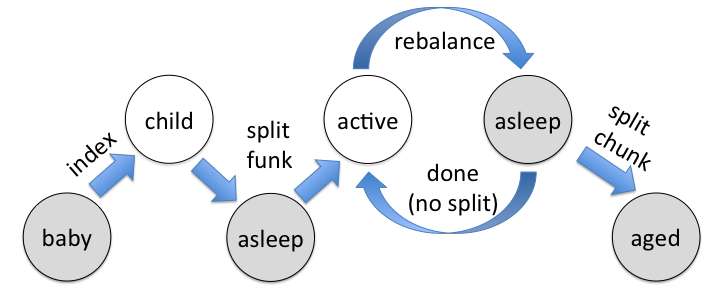
\includegraphics[width=\columnwidth]{state-diagram.png}
}
\caption{\bf{Chunk life cycle; immutable states are grey and mutable ones are white.
Chunk splits  create new chunks in immutable \emph{baby} status, which changes to the mutable \emph{child} state once they 
are indexed. When the appropriate funks are created, the chunks become \emph{active}. All rebalance operations go through an 
\emph{asleep} state when the chunk is immutable.}}
\label{fig:status}
\end{figure}
}

In case of a split, the chunk is immutable when we create two new chunks to replace it. 
If the chunk has a munk, we split the munk (by creating two new munks) and update the appropriate pointers in the new chunks.  
Since creating new funks again involves I/O, we do not wish to keep the new chunks immutable for the duration of this process,
and allow funk creation to proceed in the background while the two new chunks still point to the same old funk. 

After we replace the old chunk in the list with the two new ones, 
the old chunk is still accessible via the chunk index (even though it is no longer in the list). 
The new chunks are therefore created in \emph{baby} status, indicating that they are still immutable. 
Once the new chunks are indexed, the old chunk is \emph{aged}, and the new chunks can become mutable.
At this point, we change their status to \emph{child}, indicating that they are no longer immutable, but share a funk with another chunk,
and so should not be rebalanced. Once the funk split completes, we make the chunk immutable in order
to complete the funk switch, and then change their  status  to active. 
%The chunk's life-cycle is depicted in Figure~\ref{fig:status}.

Merges can be handled the same way by making the two merged munks immutable for the duration of the switch; we do not implement this feature in our prototype.

\subsection{Disk flushes and recovery}
\label{ssec:flush-recovery}

Like most popular KV-stores, \sys\ supports two modes of operation -- \emph{synchronous} and \emph{asynchronous}. 
With the former,  updates are persisted to disk before returning to the user, and so a user is ensured when its operation
completes that the written data will survive failures. The drawback of this approach is that it is 
roughly an order-of-magnitude slower than the asynchronous mode in  existing KV-stores like RocksDB~\cite{RocksDB} as well as in \sys. 

The asynchronous mode expedites updates by performing them in
RAM only and periodically \emph{flushing} them to disk. This reduces write latency and increases throughput, but 
may lead to loss of data that was written shortly before the crash. The tradeoffs between the two approaches are 
well known and the choice is typically left to the user.

\paragraph{Recovery semantics.}
In the synchronous mode, 
%every put operation performs a flush after writing the data in the appropriate funk's \code{log}, and then returns. 
%This ensures that 
the funks always reflect all completed updates. In this case, recovery is straightforward: we simply construct
the chunks linked list and chunk index from the funks on disk, and then the database is immediately ready to serve new requests, populating munks and Bloom filters on-demand.  

In the asynchronous mode, some suffix of the  data written before a crash may be lost, but we  
ensure that the data store \emph{consistently} reflects a \emph{prefix} of the  values written.
For example, if \code{put(k1, v1)} completes before \code{put(k2, v2)} 
is invoked and then the system crashes, then following the recovery, 
if \code{k2} appears in the data store, then \code{k1} must appear in it as well. 
%conversely, if the update of \code{k1}  is lost, \code{k2}  must be also excluded.
Such recovery to a \emph{consistent snapshot} of the data store is important, since later updates may depend on earlier ones. 

\paragraph{Checkpointing for consistent recovery.}

To support recovery to a consistent snapshot in asynchronous mode, we use a background process to
periodically create and persist \emph{checkpoints} of the data store.
The checkpointing process creates a snapshot similarly to the atomic scan mechanism. That is, 
it begins by fetching-and-incrementing GV to obtain a 
 snapshot version \code{gv}.  Next, 
it synchronizes with pending puts via PO to ensure that all puts with smaller versions are complete. 
It then flushes all the pending writes to disk (using an \code{fsync} call). 
Once the flush is complete, it writes \code{gv} to a dedicated \emph{checkpoint file} on disk,
indicating that all updates pertaining to versions smaller than or equal to this version have been persisted.
Note that some puts with higher versions than \code{gv} might be reflected on disk while others are not. 

Recovery in \sys\ is lazy, keeping all data on disk, and 
allowing it to be fetched from disk into munks  on demand in the course of the normal operation mode. 
But to ensure consistency, following a recovery,  
retrievals from funks should ignore newer versions that were not included in the latest completed checkpoint before the crash. This must be done by every operation that reads data from a funk -- \code{get} or \code{scan} from a munk-less chunk, funk rebalance,  or a munk load. 

To facilitate this check, 
we distinguish between pre-crash versions and new ones created after recovery using \emph{incarnation numbers}. Specifically, a version is split into an incarnation number (in our implementation, the four most-significant bits of the version) and a per-incarnation version number. The normal mode operation incrementing the GV in effect increases the latter. The recovery procedures increments the former and resets the latter, so 
versions in the new incarnation begin from zero. 

We maintain a \code{recoveryTable} mapping each recovered incarnation to its last checkpointed version number. 
For example, Table~\ref{table:recovery} shows a possible state of the recovery table after two recoveries, i.e., during incarnation $2$. 

\begin{table}[h]
\begin{center}
\begin{tabular}{ll}
incarnation & last checkpointed version \\
\hline
0 & 1375\\
1 &  956\\
\end{tabular}
\end{center}
\caption{Example recovery table during incarnation $2$.}
\label{table:recovery}
\end{table} 
 
Every read from a funk  (during \code{get},  \code{scan}, funk rebalance,  and munk load) then
refers to the recovery table in order to identify versions that should be ignored -- these are versions from old incarnations that exceed the checkpoint number for their incarnation. 

%\paragraph{Recovery procedure.} 
The recovery procedure is very simple: it reads the checkpoint time from disk, loads the \code{recoveryTable} into memory, adds a new row to it with the last incarnation and latest checkpoint time, and persists it again. It then increments the incarnation number, and resumes normal operation with version number $0$ in the new incarnation.




\remove{
\subsection{\sys\ operations}
\label{ssec:ops}

\inred{Consider if we want full pseudocode}
}








